\documentclass[fontsize=6pt, landscape, a4paper]{scrartcl}
\usepackage{graphicx} % Required for inserting images
\usepackage[margin=1cm]{geometry}
\usepackage[compact]{titlesec}
\usepackage{multicol}
\usepackage{listings}
\usepackage{enumitem}
\usepackage[linesnumbered,ruled,vlined]{algorithm2e}
\usepackage{tikz}
\usetikzlibrary{positioning, arrows.meta, trees}
\usepackage{amsmath, amssymb, mathtools}

% Formatting titles
\titleformat{\section}
    {\normalfont\Large\bfseries\color{blue}}
    {\thesection}{1em}{}

\titleformat{\subsection}
    {\normalfont\normalsize\itshape\bfseries}
    {\thesubsection}{1em}{}

\titleformat{\subsubsection}
    {\normalfont\small\itshape}
    {\thesubsubsection}{1em}{}

% Formatting spacing
\titlespacing*{\section}{0pt}{4pt}{2pt}
\titlespacing*{\subsection}{0pt}{3pt}{1pt}
\titlespacing*{\subsubsection}{4pt}{0pt}{0pt}

\setlength{\parindent}{0pt}
\setlength{\parskip}{0pt}
\setlist{nosep}

\definecolor{myblue}{cmyk}{1,.72,0,.38}
\everymath\expandafter{\the\everymath \color{myblue}}

% Code listing formatting
\lstset{
    basicstyle=\ttfamily\scriptsize, % Use a smaller monospace font
    aboveskip=2pt,                   % Reduce space above the block
    belowskip=2pt,                   % Reduce space below the block
    breaklines=true,                 % Automatically wrap long lines
    xleftmargin=0pt,                 % Remove left margin padding
    showstringspaces=false           % Don't show weird underscores in strings
}

\newenvironment{tightcenter}{%
  \setlength\topsep{0pt}
  \setlength\parskip{0pt}
  \begin{center}
}{%
  \end{center}
}

\begin{document}

\begin{center}
    {\Huge \textbf{CS2040S Cheatsheet}}
\end{center}

\begin{multicols*}{4}
    \raggedcolumns
    \section*{Ch1: Order of Growth}
    \subsection*{Properties}
    Let $T(n) = O(f(n))$ and $S(n) = O(g(n))$
    \begin{itemize}
        \item \textbf{Addition:} $T(n) + S(n) = O(f(n) + g(n))$
        \item \textbf{Multiplication:} $T(n) \cdot S(n) = O(f(n) \cdot g(n))$
        \item \textbf{Composition:} $T(n) \circ S(n) = O(f(n) \circ g(n))$
              \begin{itemize}
                  \item \textit{Only if both functions are increasing}
              \end{itemize}
        \item \textbf{Max:} $\max(f(n), g(n)) \leq f(n) + g(n)$
    \end{itemize}

    \subsection*{Space Complexity}
    \begin{itemize}
        \item Take the \textbf{max space} taken at any point of time
    \end{itemize}

    \begin{itemize}
        \item For example:

              \begin{lstlisting}[language=Java]
    int logN = Math.log(n);
    
    for (int i = 0; i < n; i++) {
        int[] newArray = new int[logN];
    }
    \end{lstlisting}

              \begin{itemize}
                  \item Takes up $O(\log(n))$ space instead of $O(n\cdot \log(n))$
              \end{itemize}
    \end{itemize}

    \section*{Ch2: Sorting Algorithms}
    \subsection*{Insertion Sort}
    \begin{lstlisting}
void insertionArray(int arr[], int n) {
    For each element from the first to last element
    Keep trying to shift that element if it's smaller
    than the element to the left
}
\end{lstlisting}

    \begin{itemize}
        \item \textbf{Invariant:} At the start of the $i^{th}$ iteration, the sub-array $arr[0, (i - 1)]$ is in sorted order
        \item \textbf{Time Complexity:} $O(n^{2})$
        \item \textbf{Space Complexity:} $O(1)$
    \end{itemize}

    \subsection*{Selection Sort}
    \begin{lstlisting}
void insertionSort(int arr[], int n){
    For each position i from 0 to n - 1
        Find minimum element in sub-array arr[i..(n-1)].
        Set the element at position i in arr to the minimum
        element found.
}

\end{lstlisting}

    \begin{itemize}
        \item At the beginning of the $i^{th}$ iteration, the sub-array $arr[0 \dots (i-1)]$
              is the same as the sub-array $sorted[0 \dots (i-1)]$
        \item \textbf{Time Complexity:} $O(n^{2})$
        \item \textbf{Space Complexity:} $O(1)$
    \end{itemize}

    \subsection*{Merge Sort}
    \begin{lstlisting}
void mergeSort(int arr[], int left, int right){
    if left + 1 == right:
        return;
    mid = (right - left) / 2;
    mergeSort(arr, left, mid);
    mergeSort(arr, mid, right);
    output = new int[right - left];
    merge(arr, left, right, output);
    copy from output to arr[left, right)
}

\end{lstlisting}

    \begin{itemize}
        \item At the beginning of the $i^{th}$ iteration, the sub-array $arr[0 \dots (i-1)]$
              is the same as the sub-array $sorted[0 \dots (i-1)]$
        \item \textbf{Time Complexity:} $O(n\cdot \log(n))$
        \item \textbf{Space Complexity:} $O(n)$
    \end{itemize}

    \subsection*{Quick Sort}
    \begin{lstlisting}
void quickSort(int arr[], int left, int right){
    if left + 1 == right:
        return; // empty array do nothing
        
    // partition array based on the first element of array
    pivot_idx = partition(arr, left);

    Quicksort(arr, left, pivot_idx);
    Quicksort(arr, pivot_idx + 1, right);
}

\end{lstlisting}

    \begin{itemize}
        \item At the beginning of each iteration, the elements to the left of a certain index
              $i$ are all less than or equal to the pivot ($arr[i]$) and vice versa
        \item \textbf{Time Complexity:} Depends on choice of pivot
              \begin{itemize}
                  \item Worst case: $O(n^{2})$ first/last pivot
                  \item Worst case: $O(n \cdot \log(n))$ median element
                  \item Worst case: $\infty$ random element
              \end{itemize}
        \item \textbf{Space Complexity:} $O(n)$
    \end{itemize}

    \section*{Binary Search Trees}
    \subsection*{General}
    \begin{itemize}
        \item a BST is either empty, or a node pointing to 2 BSTs
        \item Balanced tree: $h = \log_{2} n$
        \item For a full binary tree of size $n$, $\exists k \in \mathbb{Z}^{+}$ s.t. $n =
                  2^{k} -1$
    \end{itemize}

    \subsection*{Runtime for Operations}
    \begin{itemize}
        \item \textit{Lookup:} $O(n)$ when every node has a single child
              \begin{itemize}
                  \item If not, can be $O(h)$, where $h$ is the height
              \end{itemize}
        \item \textit{Insert:} $O(h)$
        \item \textit{Delete:} $O(h)$
              \begin{itemize}
                  \item Case 1: No children - remove the node
                  \item Case 2: 1 child - remove the node, connect parent to child
                  \item Case 3: 2 children - delete the successor; replace node with successor
              \end{itemize}
    \end{itemize}

    \section*{AVL Trees}
    \subsection*{General}
    \begin{itemize}
        \item Invariant: \textbf{Height balanced} (maintained with rotations)
              \begin{itemize}
                  \item $\Leftrightarrow |v.left.height - v.right.height| \leq 1$
              \end{itemize}
    \end{itemize}
    \subsection*{Rotations}
    \noindent
    \begin{minipage}{0.48\linewidth}
        \centering
        \textbf{Right (RR)} \\
        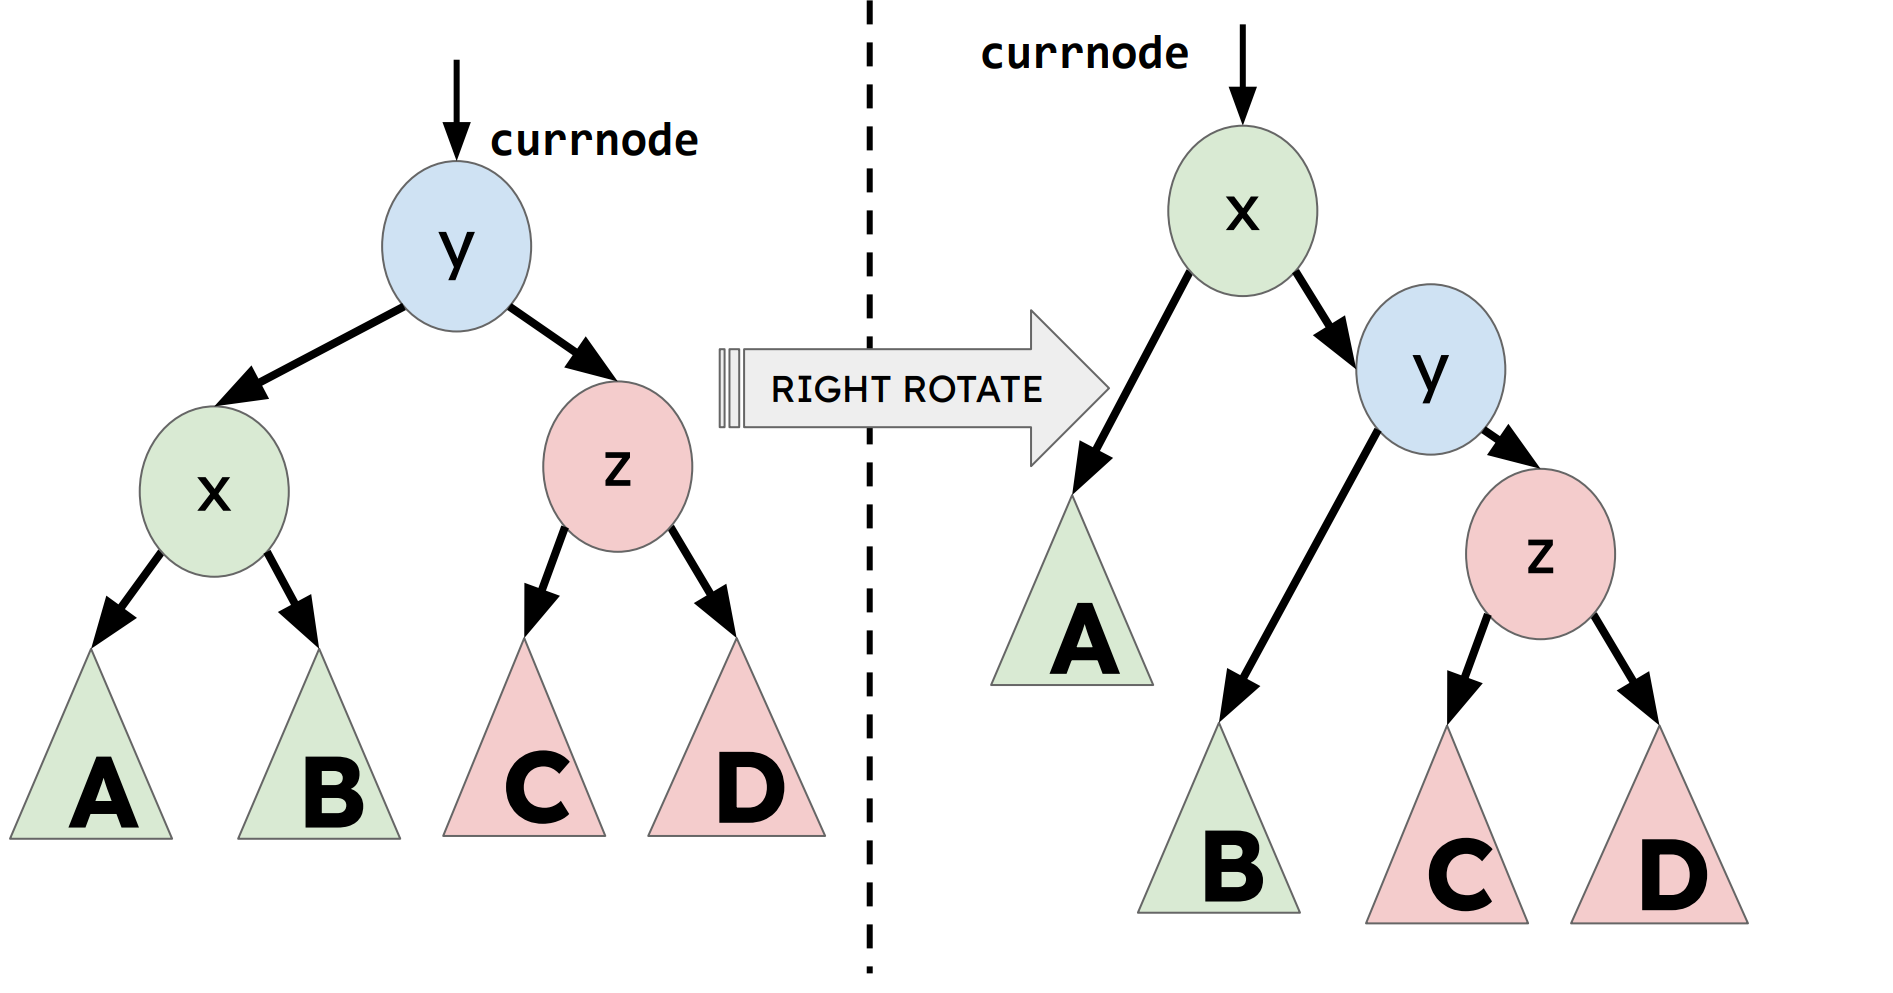
\includegraphics[width=\linewidth]{images/right_rotate.png}
        % captionof is often too bulky for cheatsheets, 
        % consider just using text if it still overflows
    \end{minipage}
    \hfill
    \begin{minipage}{0.48\linewidth}
        \centering
        \textbf{Left (LL)} \\
        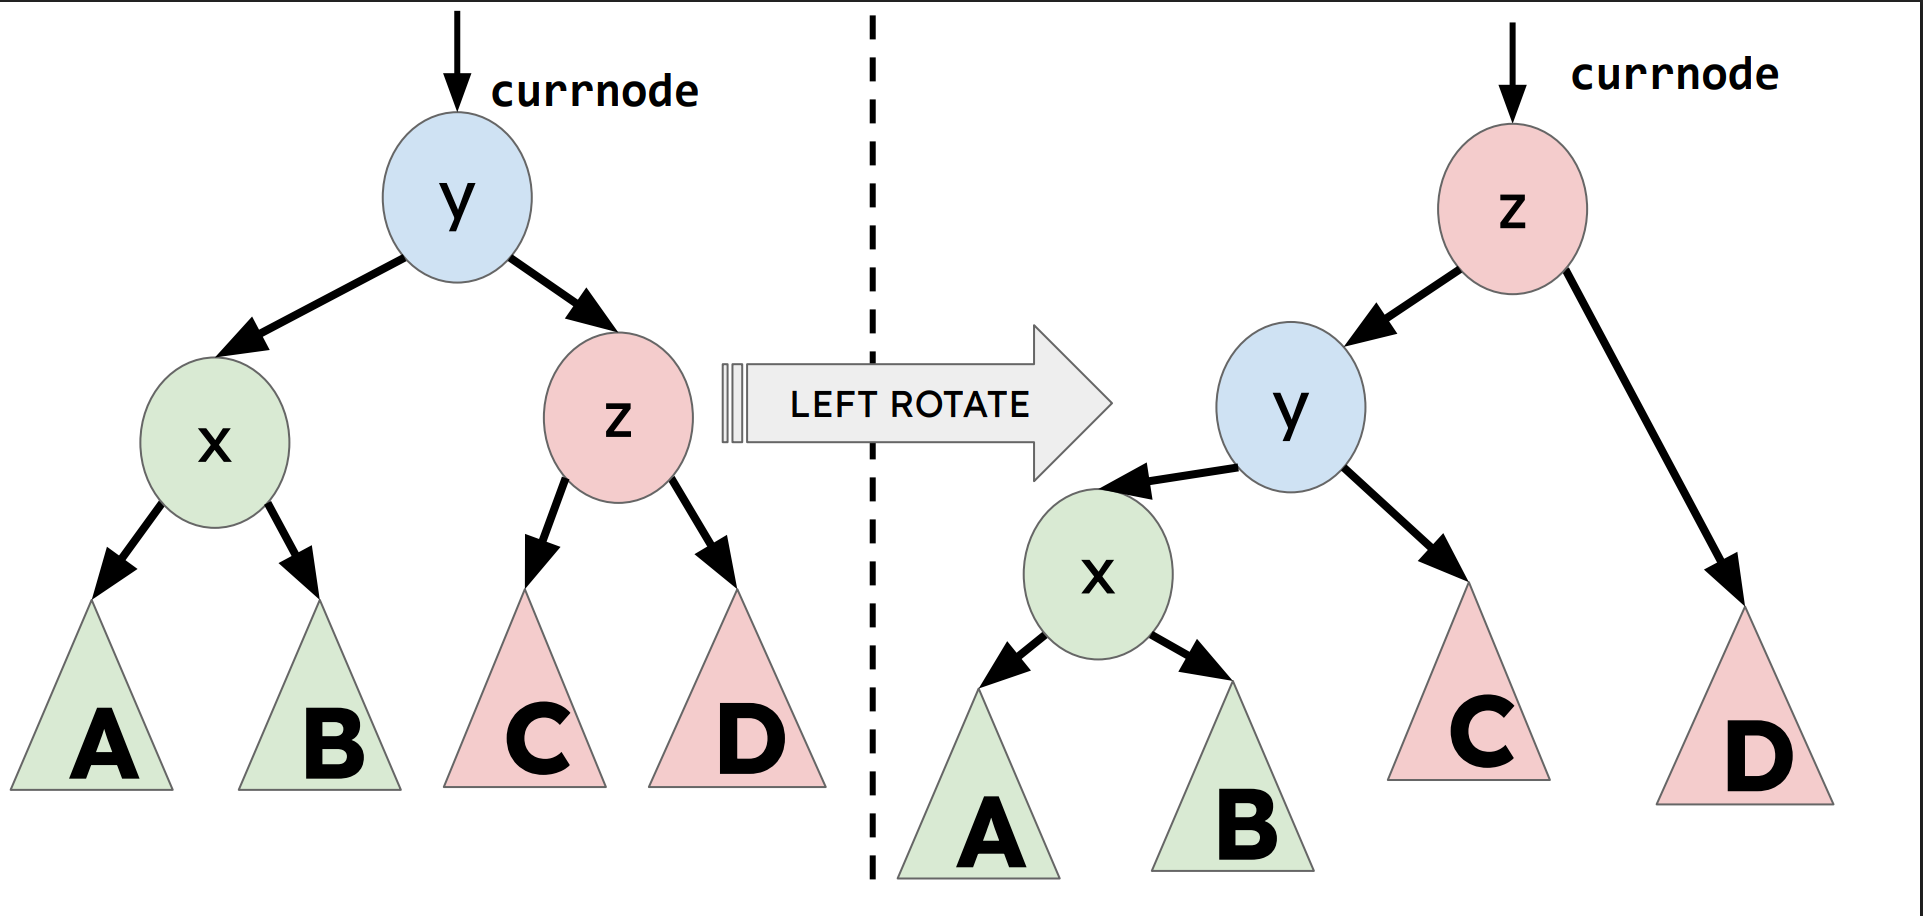
\includegraphics[width=\linewidth]{images/left_rotate.png}
    \end{minipage}
    \vspace{1em}

    \subsection*{Terminology}
    \begin{itemize}
        \item \textbf{Left/Right Heavy:} Height of left/right child node is taller than height of right/left child node
              \begin{itemize}
                  \item Perform a right/left-rotation
              \end{itemize}
    \end{itemize}
    \section*{AVL Rebalancing Cases}
    \textit{Check balance factor: $bf = \text{height}(L) - \text{height}(R)$. Rebalance if $|bf| > 1$}

    \subsection*{1. Left-Left (LL) Heavy}
    \begin{itemize}
        \item \textbf{Condition:} $y$ is left-heavy, and $y.left$ is left-heavy
        \item \textbf{Fix:} Single \textbf{Right Rotation} on $y$
    \end{itemize}

    \subsection*{2. Right-Right (RR) Heavy}
    \begin{itemize}
        \item \textbf{Condition:} $y$ is right-heavy, and $y.right$ is right-heavy
        \item \textbf{Fix:} Single \textbf{Left Rotation} on $y$
    \end{itemize}
    \begin{center}
        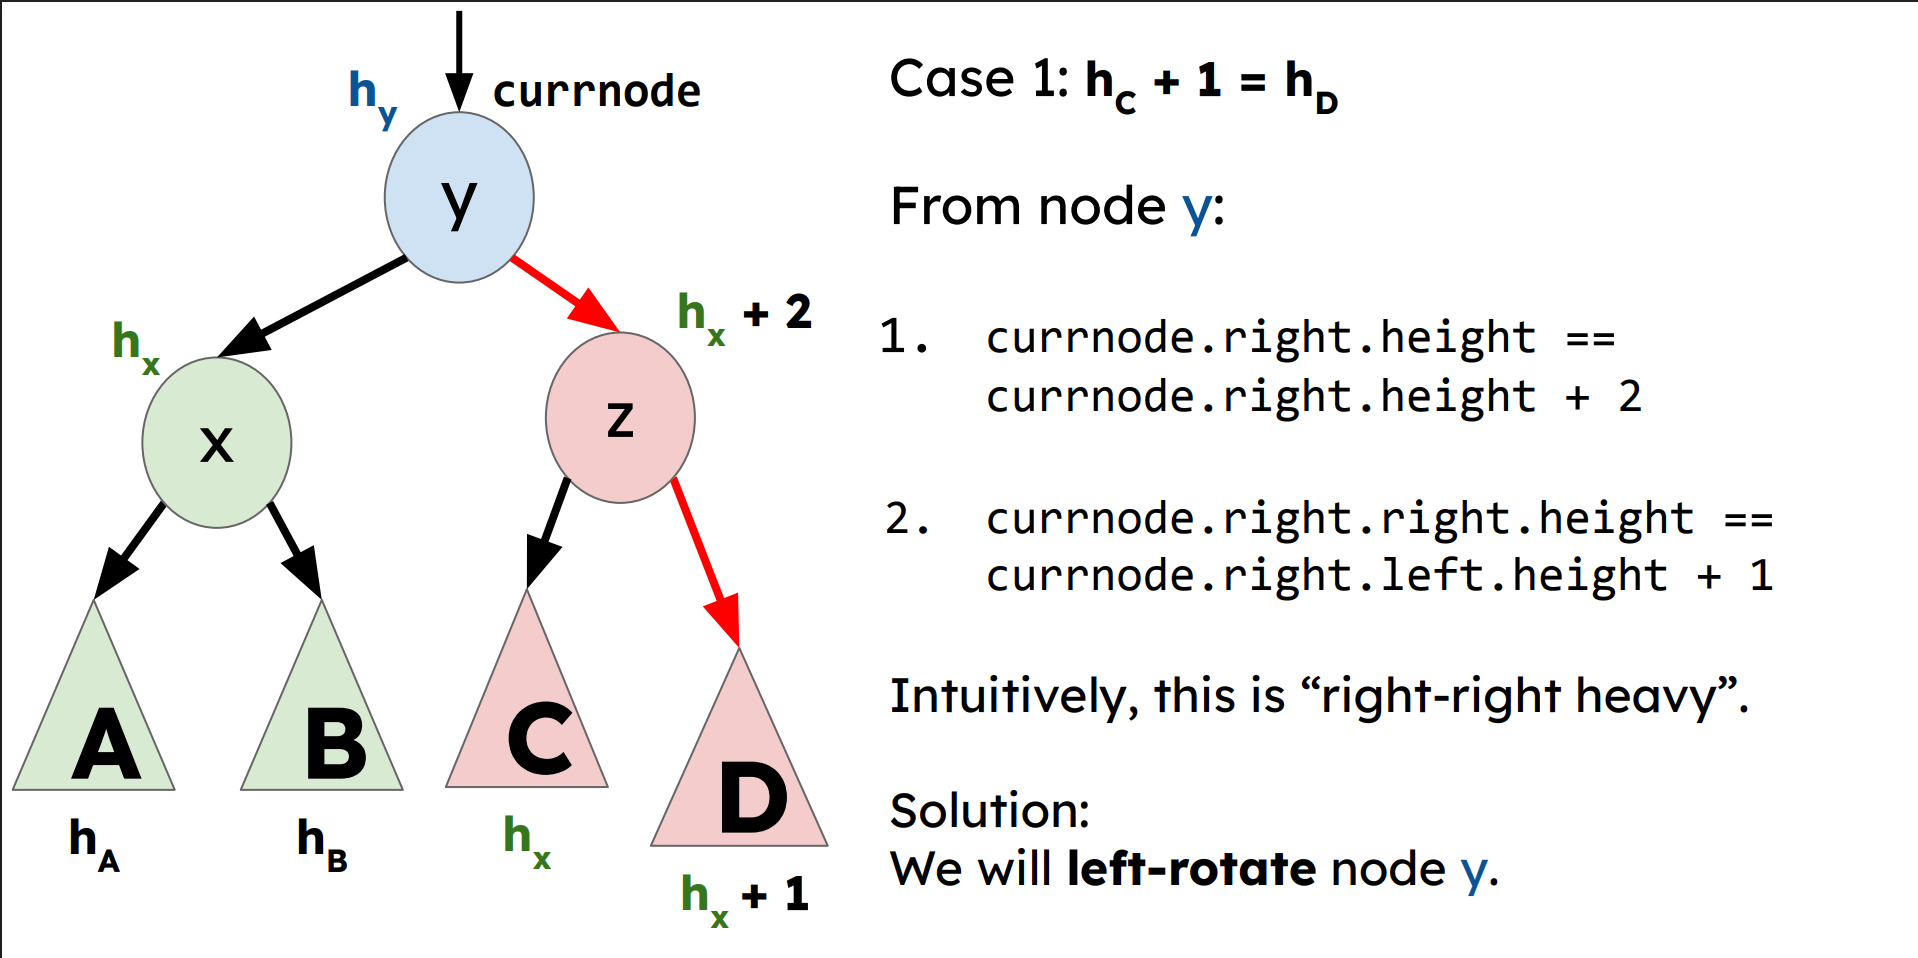
\includegraphics[width=0.8\linewidth]{images/rr_heavy.png}
    \end{center}

    \subsection*{3. Left-Right (LR) Heavy}
    \begin{itemize}
        \item \textbf{Condition:} $y$ is left-heavy, but $y.left$ is right-heavy
        \item \textbf{Fix:} \textbf{Double Rotation}: Left-rotate $y.left$, then Right-rotate $y$
    \end{itemize}

    \subsection*{4. Right-Left (RL) Heavy}
    \begin{itemize}
        \item \textbf{Condition:} $y$ is right-heavy, but $y.right$ is left-heavy
        \item \textbf{Fix:} \textbf{Double Rotation}: Right-rotate $y.right$, then Left-rotate $y$
    \end{itemize}
    \begin{center}
        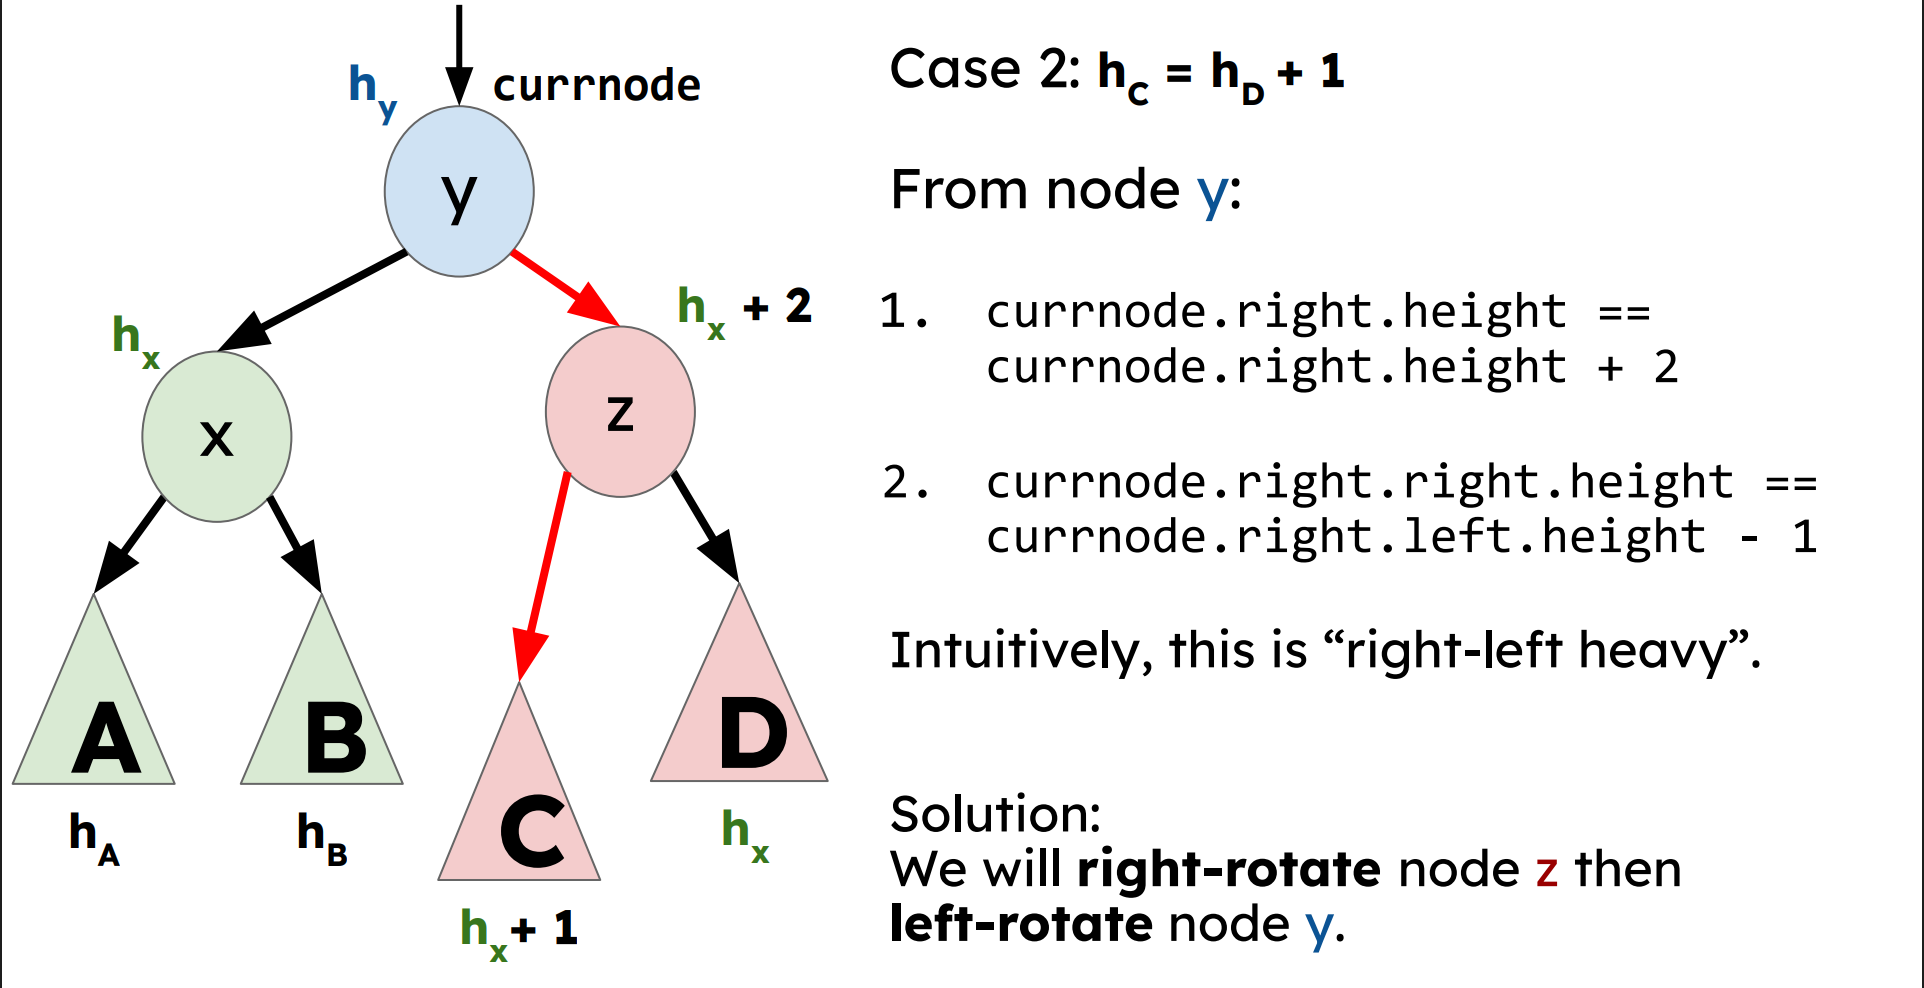
\includegraphics[width=0.8\linewidth]{images/rl_heavy.png}
    \end{center}

    \section*{Tree Augmentation Summary}
    \begin{itemize}
        \item \textbf{Size Augment:} Store subtree size to support $Rank(k)$ and $Select(i)$ in $O(h)$
        \item \textbf{Rank:} Number of elements smaller than $k$
        \item \textbf{Select:} Find key with a given rank
        \item \textbf{Maintenance:} Update $height$ and $size$ as recursion unwinds
    \end{itemize}

    \section*{AVL Deletion}
    \subsection*{1. BST Deletion Phase}
    \begin{itemize}
        \item \textbf{Leaf:} Just remove the node
        \item \textbf{1 Child:} Remove node and connect parent to the child
        \item \textbf{2 Children:} Find successor $n$ (min of right subtree), swap key with $n$, and delete $n$ (which now has $\leq 1$ child)
    \end{itemize}

    \subsection*{2. Rebalancing Phase}
    \textit{As recursion unwinds, update heights and check $bf = h_L - h_R$. If $|bf| > 1$, rebalance at the first unbalanced node $y$}

    \textbf{Case: Deleted from Right Subtree ($bf = 2$)}
    \begin{itemize}
        \item \textbf{LL Heavy:} If $h(y.L.L) \geq h(y.L.R)$, perform \textbf{Right Rotation} on $y$
        \item \textbf{LR Heavy:} If $h(y.L.L) < h(y.L.R)$, perform \textbf{Left-Rotate} $y.L$, then \textbf{Right-Rotate} $y$
    \end{itemize}

    \textbf{Case: Deleted from Left Subtree ($bf = -2$)}
    \begin{itemize}
        \item \textbf{RR Heavy:} If $h(y.R.R) \geq h(y.R.L)$, perform \textbf{Left Rotation} on $y$
        \item \textbf{RL Heavy:} If $h(y.R.R) < h(y.R.L)$, perform \textbf{Right-Rotate} $y.R$, then \textbf{Left-Rotate} $y$
    \end{itemize}

    \subsection*{Key Difference from Insertion}
    \begin{itemize}
        \item \textbf{Propagation:} While insertion requires at most one rebalance, \textbf{deletion can trigger rebalancing at multiple levels} up to the root.
        \item \textbf{Complexity:} $O(\log n)$ for all cases
    \end{itemize}

    \section*{Hash Tables}
    \begin{itemize}
        \item Insert, delete, and lookup should run in expected $O(1)$ time, and size in
              worst-case $O(1)$ time.
    \end{itemize}

    \subsection*{Hash Function}
    \begin{itemize}
        \item \textbf{Load Factor ($\alpha$):} $n/m$, representing the expected length of a chain.
        \item \textbf{Criteria for a Good Hash Function:} Must evaluate deterministically, look random for new inputs, and execute efficiently.
        \item \textbf{Simple Uniform Hashing Assumption (SUHA):} Assumes each new key picks any table index uniformly at random, ensuring keys are distributed evenly. If $n/m = O(1)$, expected runtime of operations is $O(1)$.
        \item \textbf{Division Method:} $h(k) = k \bmod m$ (choose prime $m$, avoid $m=2^{x}$)
        \item \textbf{Multiplication Method:} $h(k) = (Ak) \bmod 2^{w} \gg (w-r)$
    \end{itemize}

    \subsection*{Collision Resolution}
    \begin{itemize}
        \item \textbf{Separate Chaining}
              \begin{itemize}
                  \item Each slot in the table acts as a head for a linked list.
                  \item \textbf{Worst-Case Runtime:} $O(n)$ for insert, lookup, and delete if all items collide into a single list.
                  \item \textbf{Expected Runtime (SUHA):} $O(n/m)$ for insert, lookup, and delete.
              \end{itemize}

        \item \textbf{Open Addressing (Linear Probing)}
              \begin{itemize}
                  \item Stores key-value pairs directly within the table array itself.
                  \item \textbf{Mechanism:} If an index is occupied, sequentially try the next slot until an empty one is found.
                  \item \textbf{Worst-Case Runtime:} $O(n)$ for insert, lookup, and delete.
                  \item \textbf{Expected Runtime (SUHA):} $O(1)$ for insert, lookup, and delete.
                  \item \textbf{Deletion Constraints:} Simply removing an item breaks the search ``run'' for subsequent keys.
                  \item \textbf{Deletion Fix (Shifting):} When removing at index $i$, check subsequent items $e$. If $i$ is within $e$'s target interval, move $e$ to index $i$.
                  \item \textbf{Interval Cases:}
                        \begin{itemize}
                            \item Case 1 (No wrap): If $h(e) \leq \text{index}$, the interval is $[h(e),
                                              \text{index}]$.
                            \item Case 2 (Wraparound): If $h(e) > \text{index}$, the interval is $[h(e), m - 1]$
                                  and $[0, \text{index}]$.
                        \end{itemize}
              \end{itemize}

        \item \textbf{Double Hashing}
              \begin{itemize}
                  \item $(h(k, i) = f(k) + i \cdot g(k)) \bmod m$
                        \begin{itemize}
                            \item $k$: The key that is being inserted or searched for
                            \item $i$: The probe attempt number (starts at $0$, then $1, 2, 3, \dots$)
                            \item $f(k)$: The primary hash function to give your starting idx
                            \item $g(k)$: The secondary hash function to give step size
                            \item $m$: Total size of hash table
                        \end{itemize}
              \end{itemize}
    \end{itemize}

    \section*{Advanced Trees}
    \subsection*{(a, b)-trees \& B-Trees}
    \begin{itemize}
        \item \textbf{B-Tree:} A $(B, 2B)$-tree is an $(a, b)$-tree where $a=B$ and $b=2B$
        \item \textbf{Rules:}
              \newline \vspace{5pt}
              \begin{minipage}{\linewidth}
                  \begin{tabular}{|c|c|c|c|c|}
                      \hline
                                & \multicolumn{2}{c|}{\# keys} & \multicolumn{2}{c|}{\# children}
                      \\\hline
                      node type & min                          & max                              & min & max
                      \\\hline
                      root      & $1$                          & $b-1$                            & $2$ & $b$
                      \\\hline
                      internal  & $a-1$                        & $b-1$                            & $a$ & $b$
                      \\\hline
                      leaf      & $a-1$                        & $b-1$                            & $0$ & $0$
                      \\\hline
                  \end{tabular}
              \end{minipage}
              \begin{itemize}
                  \item $(a, b)$-child policy: $2 \leq a \leq (b+1)/2$
                  \item Internal node has 1 more child than its number of keys
                  \item All leaf nodes must be at the \textbf{same depth} from the root
              \end{itemize}
        \item \textbf{Heights:} Max $O(\log_a n) + 1$, Min $O(\log_b n)$
        \item \textbf{Operations:} \textit{Search, Insert, Delete} are all $O(\log n)$
              \begin{itemize}
                  \item \textbf{Split:} When a node has too many children (move median key to parent)
                  \item \textbf{Merge/Share:} When a node becomes empty during deletion
              \end{itemize}
    \end{itemize}

    \subsection*{Trie}
    \begin{itemize}
        \item \textbf{Search, Insert:} $O(L)$ for a string of length $L$
        \item \textbf{Space:} $O(\text{size of text} \cdot \text{overhead})$
    \end{itemize}

    \subsection*{kd-Tree}
    \begin{itemize}
        \item Stores geometric data (points in an $(x, y)$ plane)
        \item Alternates splitting (partitioning) via $x$ and $y$ coordinates
        \item \textbf{Construct:} $O(n \log n)$
        \item \textbf{Search:} $O(h)$
        \item \textbf{SearchMin:} $T(n) = 2T(n/4) + O(1) \implies O(\sqrt{n})$
    \end{itemize}

    \subsection*{Merkle Trees}
    \begin{itemize}
        \item Binary tree - nodes augmented with a hash of their children
        \item Same root value $\implies$ identical tree
    \end{itemize}
    \begin{center}
        \begin{minipage}{0.64\linewidth}
            \vspace{5pt}
            \textbf{Merkle Tree} \\
            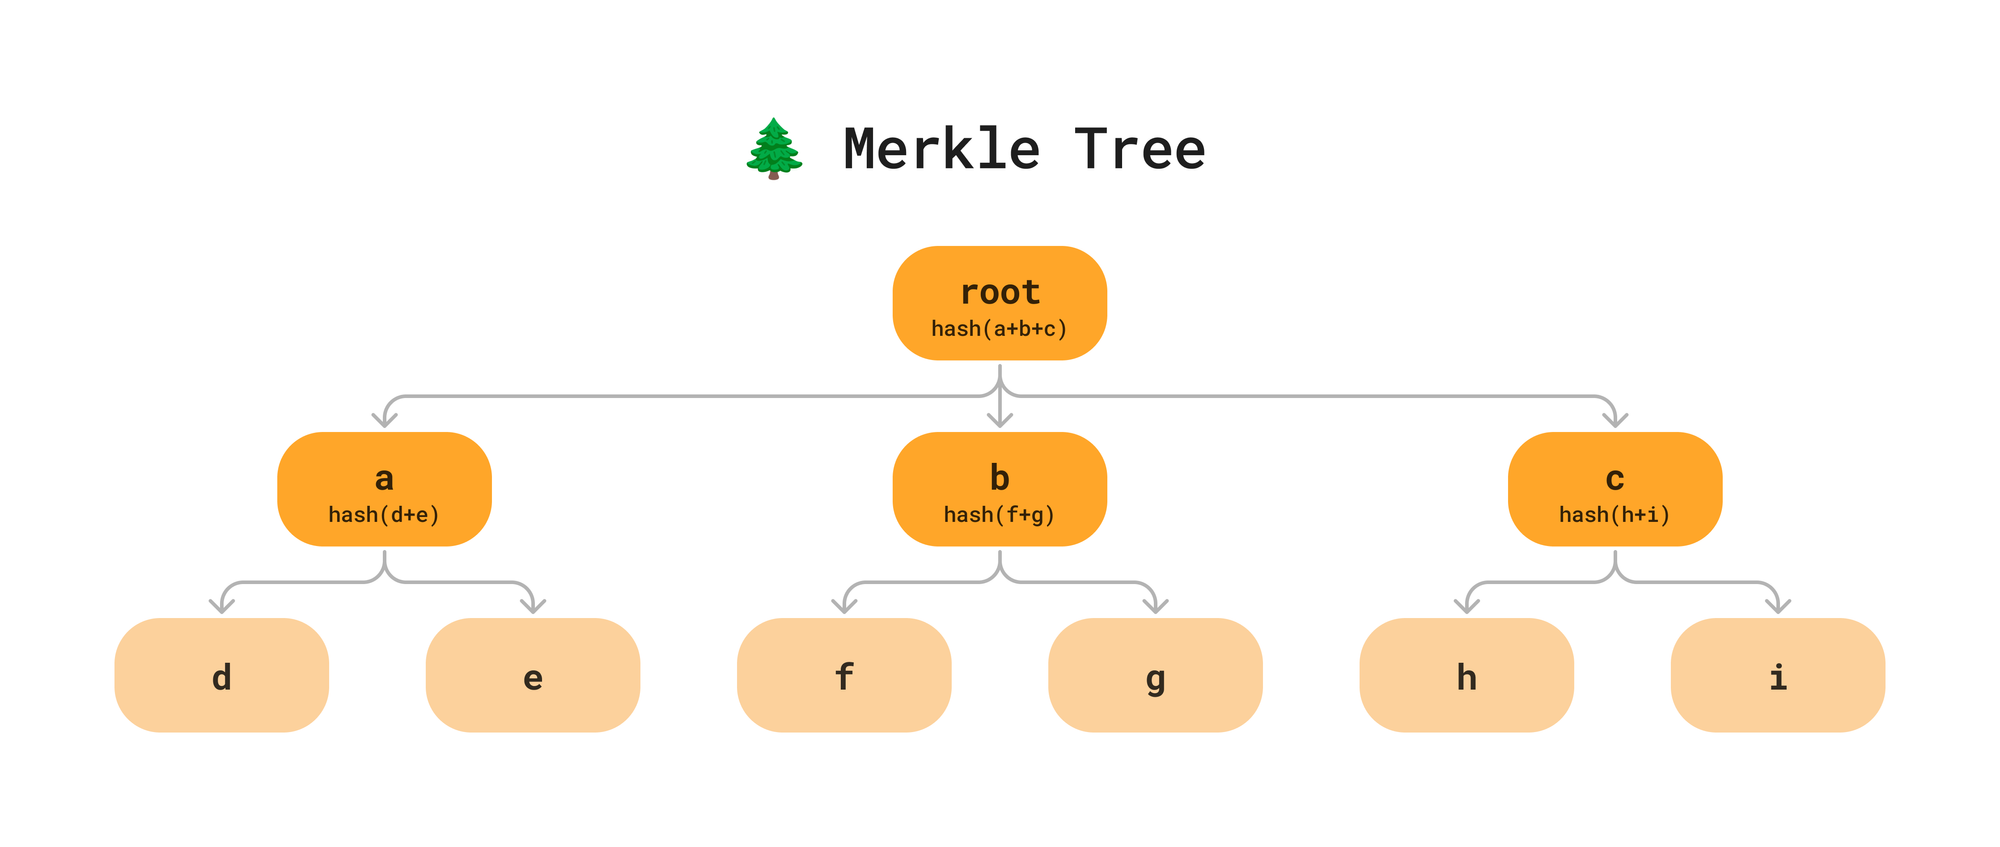
\includegraphics[width=0.8\linewidth]{images/merkle.png}
        \end{minipage}
    \end{center}

    \section*{Binary Heaps}
    \subsection*{General}
    \begin{itemize}
        \item Visualised in the form of a complete binary tree
              \begin{itemize}
                  \item Every node has either $0$, $1$, or $2$ children
                  \item Every level \textbf{must be full} except the last level
                  \item Last Level must be filled from left to right
              \end{itemize}

        \item Priorities of children are $\geq$ priority of parents (min heap)

        \item Use array to represent the tree

              \begin{minipage}{\linewidth}
                  \begin{center}
                      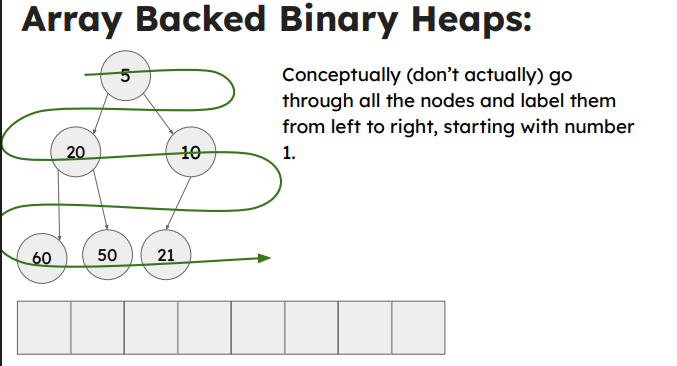
\includegraphics[width=0.8\linewidth]{images/binary_heap_array.png}
                  \end{center}
              \end{minipage}

        \item Make sure array is 1-indexed
        \item Tree traversal in array
              \begin{itemize}
                  \item Go to left child: $idx \times 2$
                  \item Go to right child: $idx \times 2 + 1$
                  \item Go to parent: $\lfloor idx \div 2 \rfloor$
              \end{itemize}

        \item To store values, we use 2 more arrays
              \begin{itemize}
                  \item id\_to\_pos
                  \item pos\_to\_id

                        \begin{minipage}{\linewidth}
                            \begin{center}
                                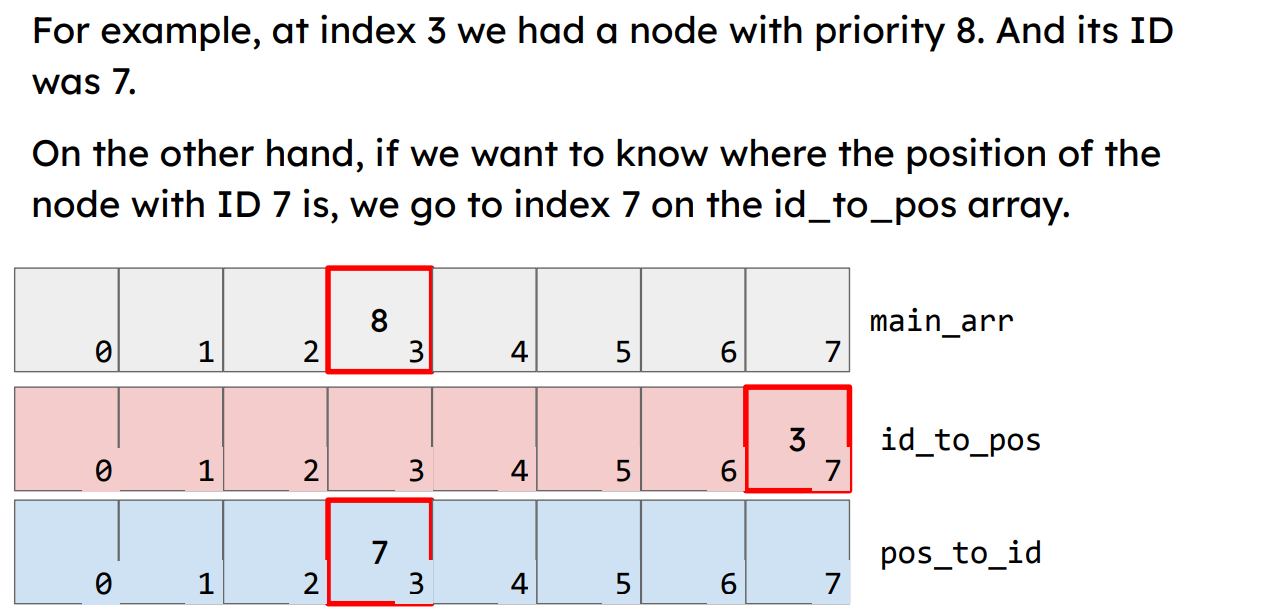
\includegraphics[width=0.8\linewidth]{images/binary_heap_triple_array.png}
                            \end{center}
                        \end{minipage}

                  \item For swaps
                        \begin{enumerate}
                            \item Swap in main array and store idx
                            \item Find id from pos\_to\_id array
                            \item Swap in the pos\_to\_id array
                            \item Use the id from step 2 to make the swap in id\_to\_pos array
                        \end{enumerate}
              \end{itemize}
    \end{itemize}

    \subsection*{Insertion}
    \begin{minipage}{\linewidth}
        \begin{center}
            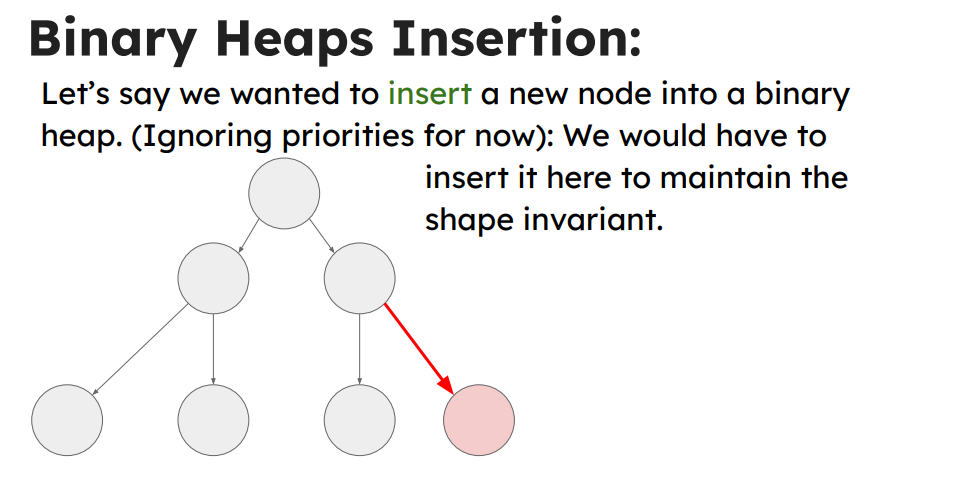
\includegraphics[width=0.8\linewidth]{images/binary_heap_insertion.png}
        \end{center}
    \end{minipage}

    \begin{enumerate}
        \item Insert at the end of the heap
        \item Keep swapping with parent node if parent node's priority is greater than
              current node
    \end{enumerate}

    \subsection*{Deletion}
    \begin{enumerate}
        \item Swap the node you want to delete with the last node
        \item Delete the last node (the node you want to delete)
        \item Compare the newly swapped node with its new parent
              \begin{itemize}
                  \item If it violates heap property, bubble up
                  \item Otherwise, bubble down
              \end{itemize}
    \end{enumerate}

    \subsection*{Extract Min}
    \begin{enumerate}
        \item Swap root node with last node
        \item Remove the last node and return
        \item Bubble the root node down if it violates binary heap invariant with the smaller
              priority child
    \end{enumerate}

    \subsection*{Heapify (Bubble Down / Sift Down)}
    \begin{enumerate}
        \item Shift all elements by 1 to make it 1-indexed
        \item Compare the current node's priority with its children for idx from $(size \div
                  2)$ to $1$
        \item If it violates the binary heap invariant, swap it with the highest-priority
              child (e.g., the smaller child in a Min-Heap)
        \item Repeat this process on the node's new position until the invariant is restored
              or it becomes a leaf node
    \end{enumerate}

    \section*{Graphs}
        \subsection*{Adjacency Matrix}
        \begin{minipage}[t]{0.48\linewidth}
            \begin{center}
                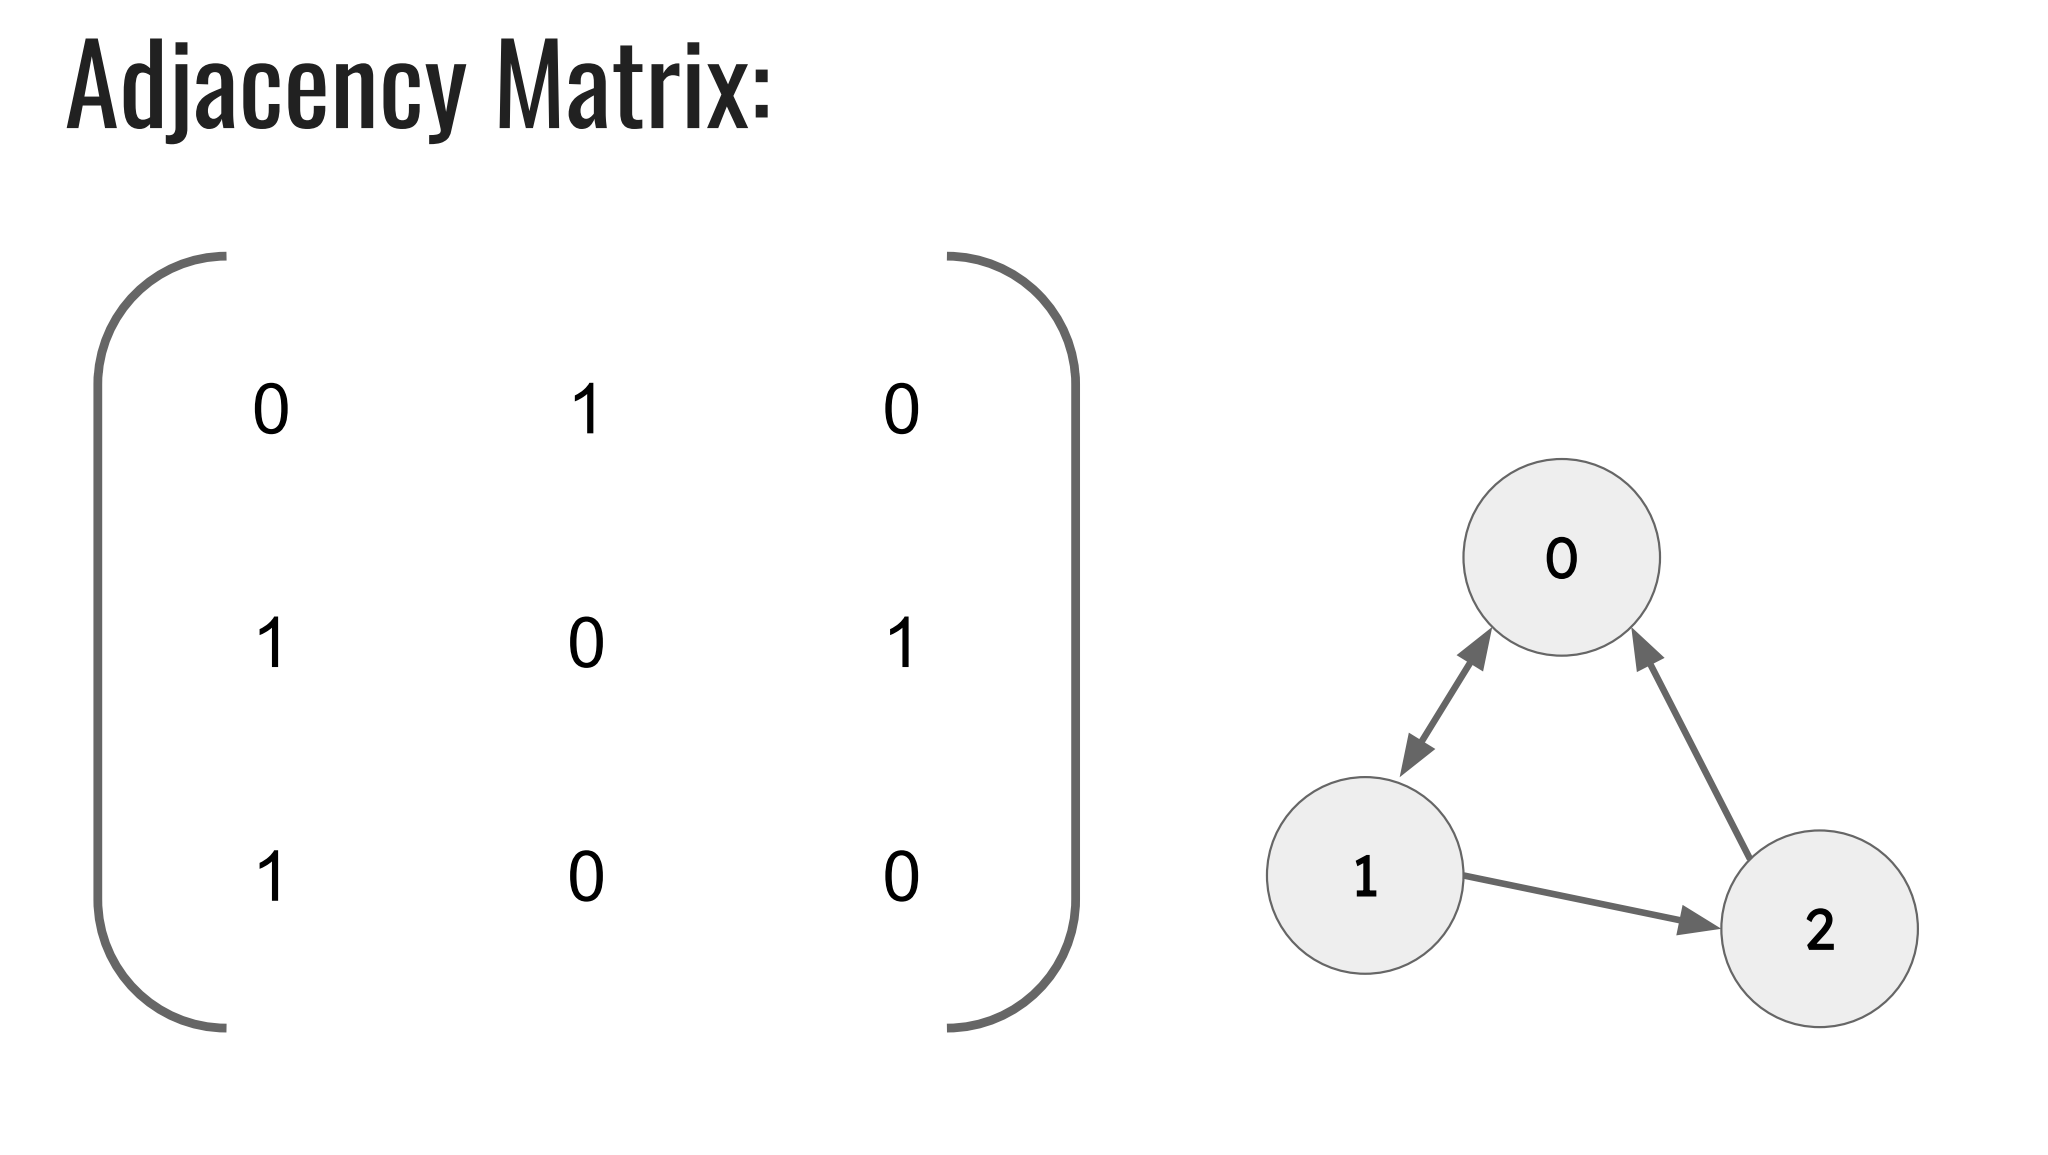
\includegraphics[width=0.8\linewidth]{images/adjacency_matrix.png}
            \end{center}
        \end{minipage}

        \begin{itemize}
            \item arr[i][j] gives the weight (1 if unweighted) of the edge from $i$ to $j$ (or 0 if no edge)
        \end{itemize}

        \subsection*{Adjacency List}
        \begin{minipage}[t]{0.48\linewidth}
            \begin{center}
                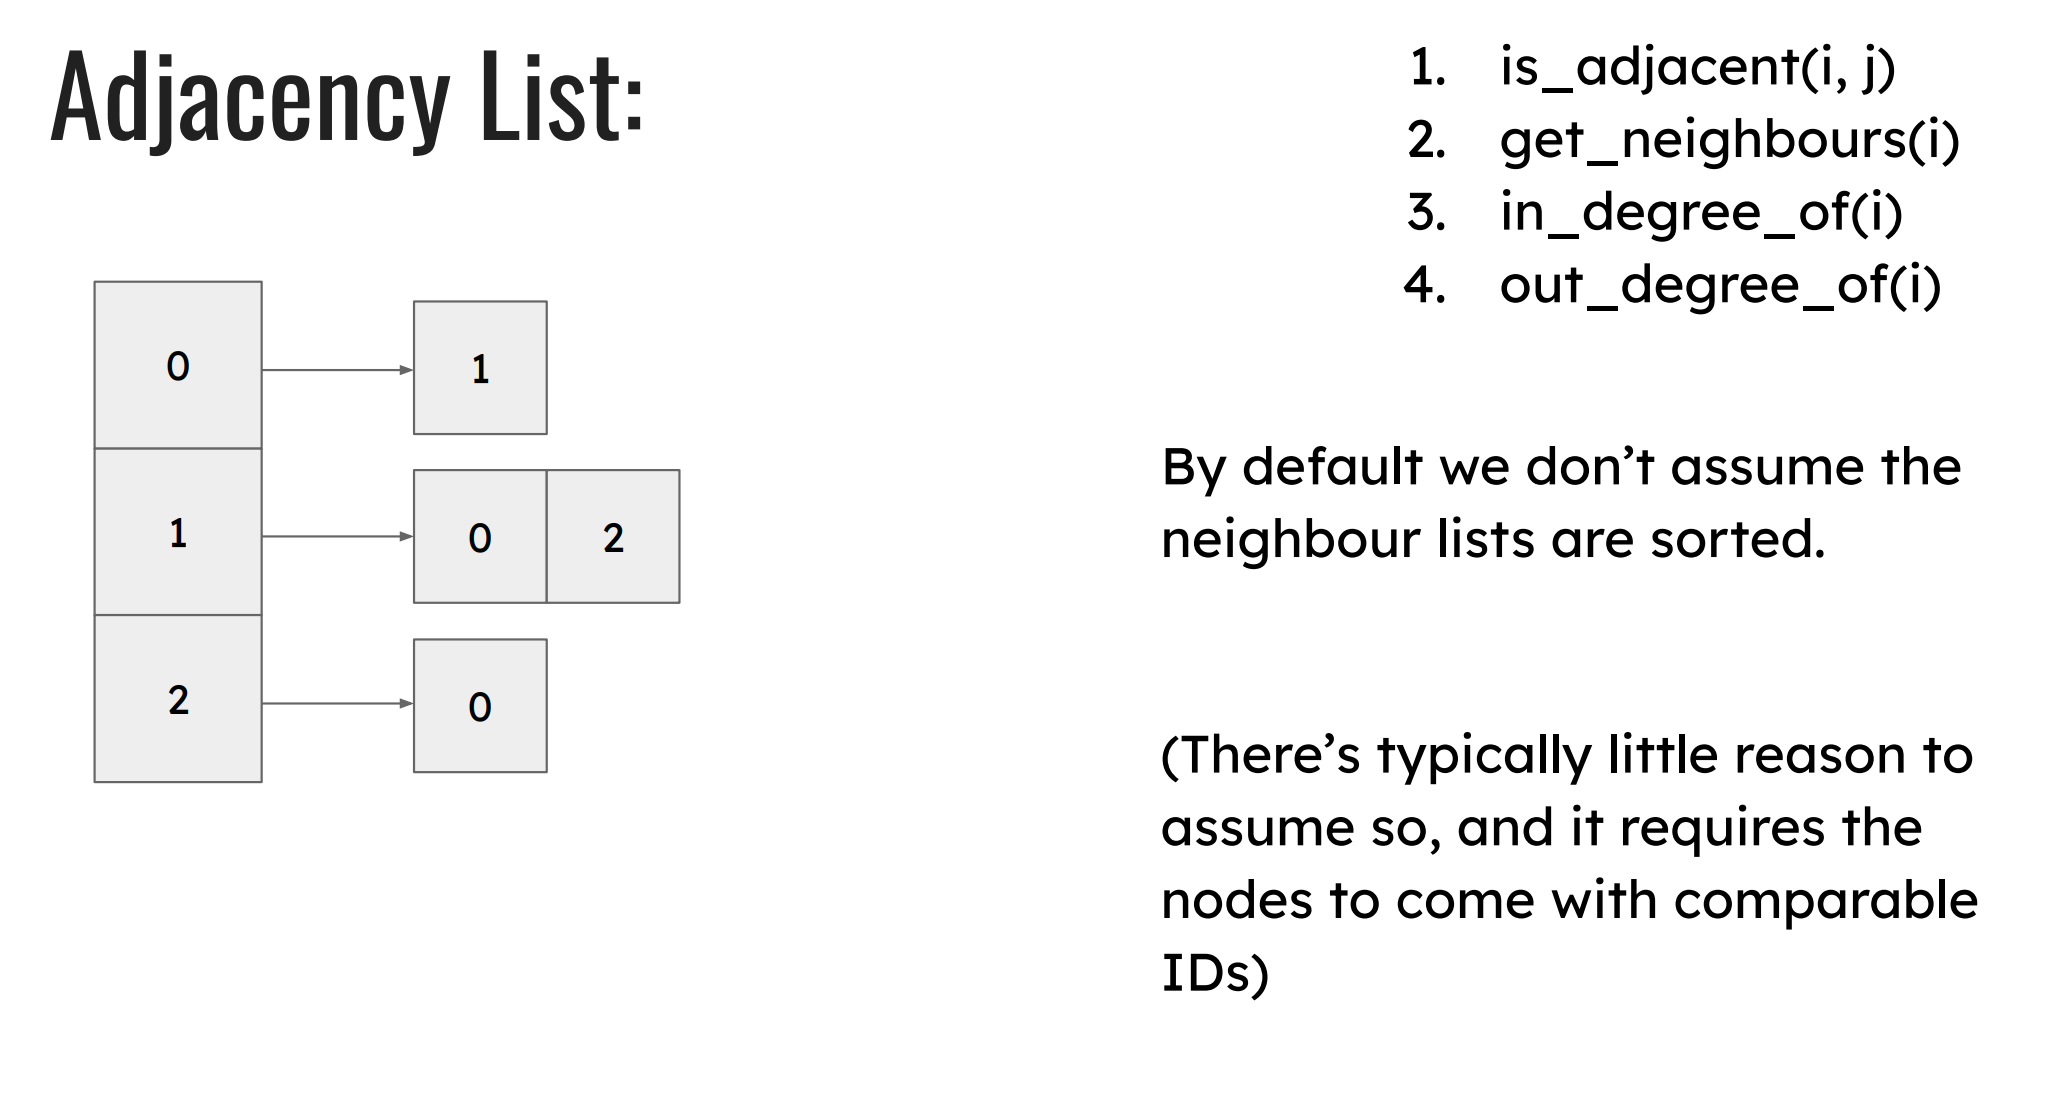
\includegraphics[width=0.8\linewidth]{images/adjacency_list.png}
            \end{center}
        \end{minipage}

        \subsection*{Edge List}
        \begin{minipage}{0.48\linewidth}
            \begin{center}
                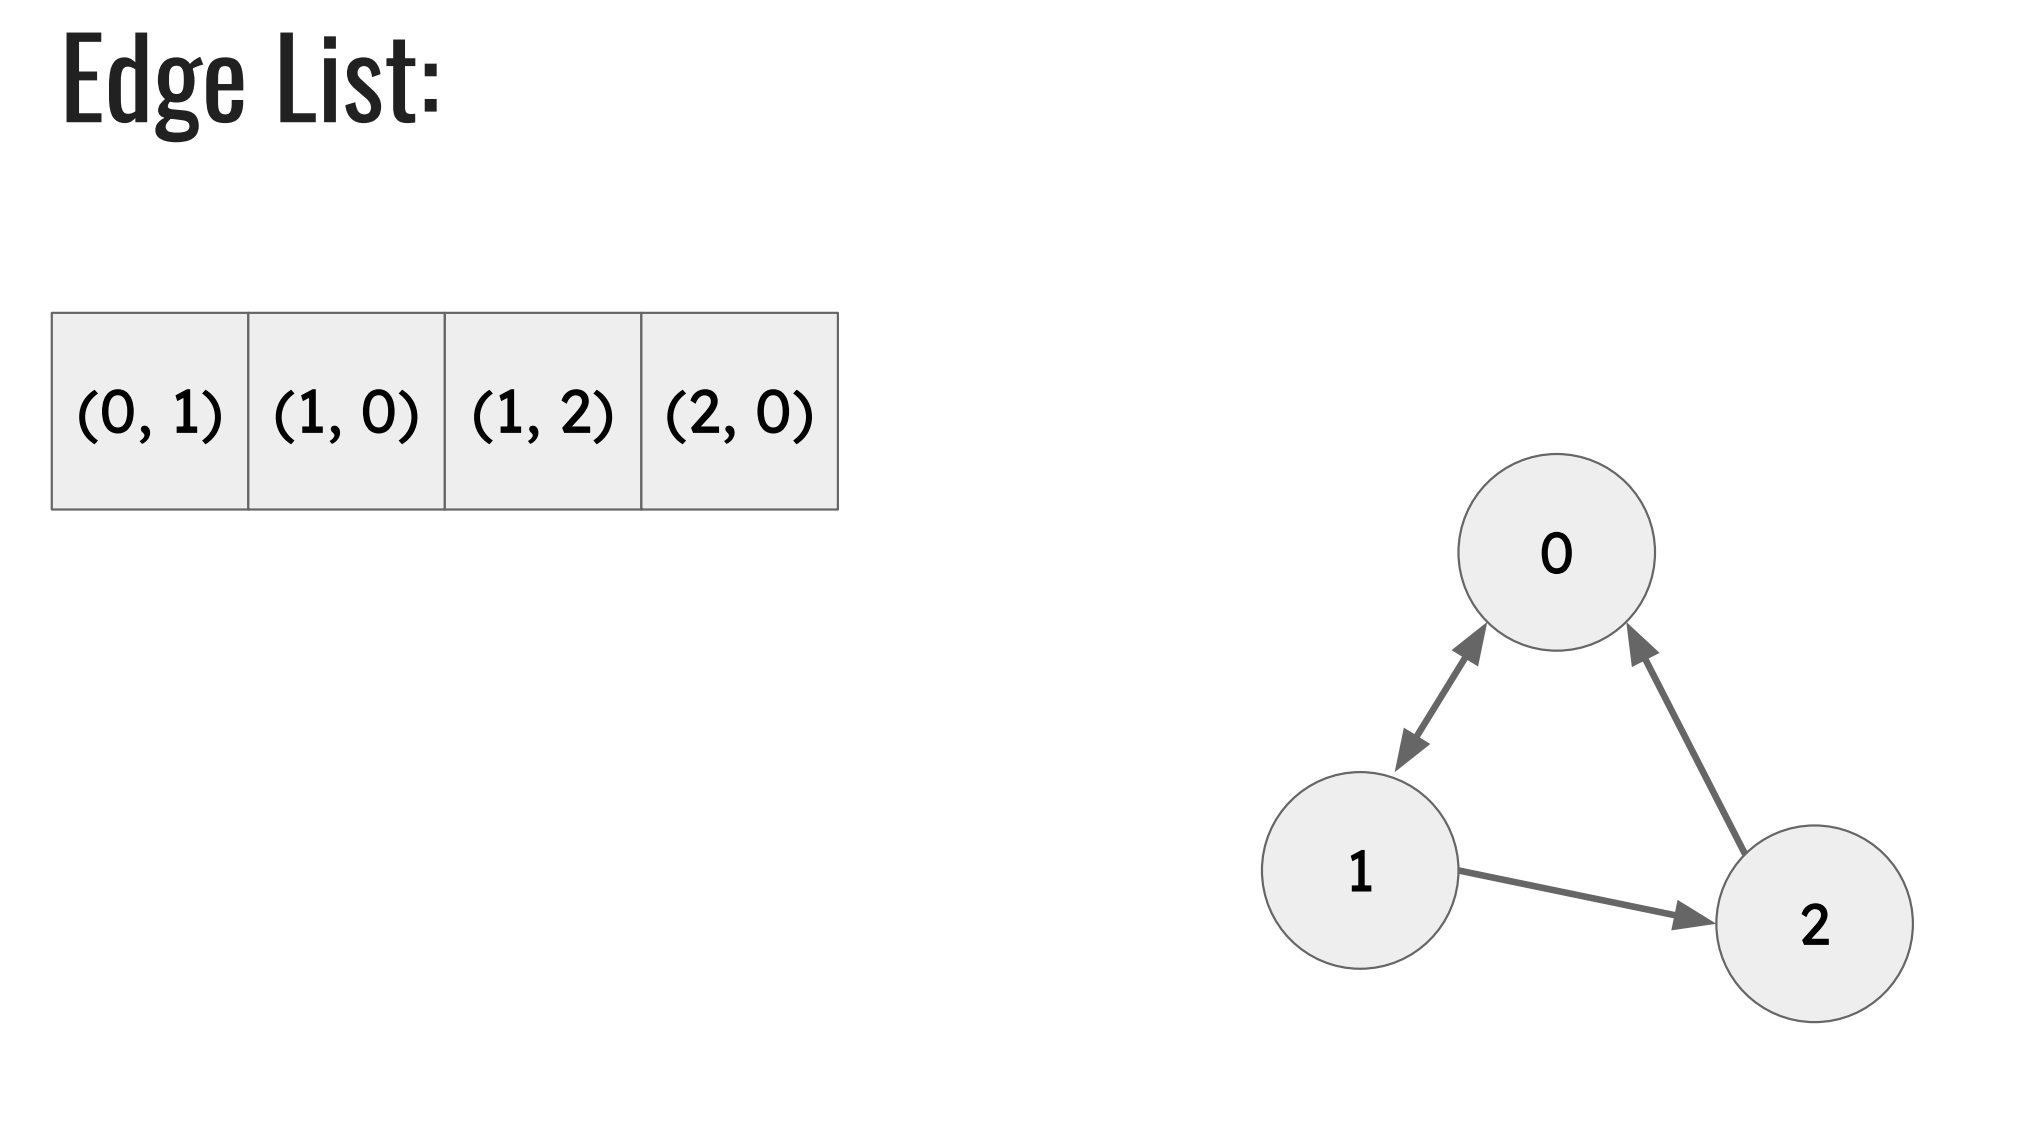
\includegraphics[width=0.8\linewidth]{images/edge_list.png}
            \end{center}
        \end{minipage}

        \begin{itemize}
            \item If edges are weighted, store as triplets $(u, v, weight)$
        \end{itemize}

        \begin{tightcenter}
            \begin{tabular}{|c|c|c|c|}
                \hline
                & \textbf{AM} & \textbf{AL} & \textbf{EL} \\
                \hline
                \textbf{is\_adj} & $O(1)$ & $O(\deg i)$ & $O(m)$ \\
                \hline
                \textbf{get\_neigh} & $O(n)$ & $O(1)$ & $O(m)$ \\
                \hline
                \textbf{in\_deg} & $O(n)$ & $O(n+m)$ & $O(m)$ \\
                \hline
                \textbf{out\_deg} & $O(n)$ & $O(1)$ & $O(m)$ \\
                \hline
                \textbf{space} & $O(n^{2})$ & $O(n+m)$ & $O(m)$ \\
                 \hline
            \end{tabular}
        \end{tightcenter}

        \subsection*{Searching}
            \subsubsection*{Breadth-First Search (BFS)}   
            \begin{itemize}
                \item Uses a queue to explore the graph level by level
                \item Time Complexity: $O(n + m)$
                \item Space Complexity: $O(n)$
            \end{itemize}

            \subsubsection*{Depth-First Search (DFS)}   
            \begin{itemize}
                \item Uses a stack to explore the graph as far as possible along each branch before backtracking
                \item Time Complexity: $O(n + m)$
                \item Space Complexity: $O(n)$
            \end{itemize}

    \section*{Appendix}
    \begin{tightcenter}
        $
            \begin{array}{| c | c | c | c | c | c |}
                \hline\textbf{sort} & \textbf{best} & \textbf{average} & \textbf{worst} & \textbf{stable?} & \textbf{memory}
                \\\hline\text{bubble} & \Omega(n) & O(n^{2}) & O(n^{2}) & \checkmark & O(1)
                \\\hline\text{selection} & \Omega(n^{2}) & O(n^{2}) & O(n^{2}) & \times & O(1)
                \\\hline\text{insertion} & \Omega(n) & O(n^{2}) & O(n^{2}) & \checkmark & O(1)
                \\\hline\text{merge} & \Omega(n\log n) & O(n\log n) & O(n\log n) & \checkmark & O(n)
                \\\hline\text{quick} & \Omega(n\log n) & O(n\log n) & O(n^{2}) & \times & O(1)
                \\\hline\text{heap} & \Omega(n\log n) & O(n\log n) & O(n\log n) & \times & O(1)
                \\\hline
            \end{array}
        $ \\
        \begin{tabular}{| c | c |}
            \multicolumn{2}{c}{sorting invariants}
            \\\hline\textbf{sort} & \textbf{invariant} (after $k$ iterations)
            \\\hline bubble & largest $k$ elements are sorted
            \\\hline selection & smallest $k$ elements are sorted
            \\\hline insertion & first $k$ slots are sorted
            \\\hline merge & given subarray is sorted
            \\\hline quick & partition is in the right position
            \\\hline
        \end{tabular} \begin{tabular}{| c | c |}
            \multicolumn{2}{c}{searching}         \\\hline
            \textbf{search} & \textbf{average}    \\\hline
            linear          & $O(n)$              \\\hline
            binary          & $O(\log n)$         \\\hline
            quickSelect     & $O(n)$              \\\hline
            interval        & $O(\log n)$         \\\hline
            all-overlaps    & $O(k\log n)$        \\\hline
            1D range        & $O(k + \log n)$     \\\hline
            2D range        & $O(k + \log^{2} n)$ \\\hline
        \end{tabular}

        data structures assuming $O(1)$ comparison cost \\* \begin{tabular}{| c | c | c |}\hline
            \textbf{data structure} & \textbf{search}                                  & \textbf{insert}       \\\hline
            sorted array            & $O(\log n)$                                      & $O(n)$                \\\hline
            unsorted array          & $O(n)$                                           & $O(1)$                \\\hline
            linked list             & $O(n)$                                           & $O(1)$                \\\hline
            tree (kd/(a, b)/binary) & $O(\log n)$ or $O(h)$                            & $O(\log n)$ or $O(h)$ \\\hline
            trie                    & $O(L)$                                           & $O(L)$                \\\hline
            heap                    & $O(\log n)$ or $O(h)$                            & $O(\log n)$ or $O(h)$ \\\hline
            dictionary              & $O(\log n)$                                      & $O(\log n)$           \\\hline
            symbol table            & $O(1)$                                           & $O(1)$                \\\hline
            chaining                & $O(n)$                                           & $O(1)$                \\\hline
            open addressing         & \multicolumn{1}{c|}{$\frac{1}{1-\alpha} = O(1)$} & $O(1)$                \\\hline
            priority queue          & (contains) $O(1)$                                & $O(\log n)$           \\\hline
            skip list               & $O(\log n)$                                      & $O(\log n)$           \\\hline
        \end{tabular}

        \vspace{1em} % Adds a little breathing room after the table
        Orders of Growth \\*
        $1 < \log n < \sqrt{n} < n < n \log n < n^{2} < n^{3} < 2^{n} < 2^{2n}$ \\*
        $\log_a n < n^{a} < a^{n} < n! < n^{n}$

        \vspace{1em}
        Orders of Growth
        \begin{align*}
            T(n) & = 2T\left(\frac{n}{2}\right) + O(n) & \implies O(n \log n)
            \\ T(n) & = T\left(\frac{n}{2}\right) + O(n) & \implies O(n)
            \\ T(n) & = 2T\left(\frac{n}{2}\right) + O(1) & \implies O(n)
            \\ T(n) & = T\left(\frac{n}{2}\right) + O(1) & \implies O(\log n)
            \\ T(n) & = 2T(n - 1) + O(1) & \implies O(2^{n})
            \\ T(n) & = 2T\left(\frac{n}{2}\right) + O(n \log n) & \implies O(n(\log n)^{2})
            \\ T(n) & = 2T\left(\frac{n}{4}\right) + O(1) & \implies O(\sqrt{n})
            \\ T(n) &= T(n - c) + O(n) &\implies O(n^{2})
        \end{align*}
    \end{tightcenter}
\end{multicols*}
\end{document}